% !TEX spellckeck=en_GB

\section{Recurrent Neural Networks}\label{sec:rnn}

\subsection{Introduction to recurrent neural networks}

The recurrent neural network (RNN) models a unit that has "memory". The memory is encoded as a state variable which is ordinarily concatenated with the input when the network predicts. The model predictions enact a sequence which has led to applications in the generation of text, time series predictions and other serialized applications. RNNs were first discussed in a theoretical paper by Jordan, MI in 86' but implemented in the modern temporal sense by \citet{Pearlmutter1989}. A simple graphical representation of the RNN cell is presented in figure \ref{fig:rnn}


\begin{figure}[h]
\centering
\tikzset{every picture/.style={line width=0.75pt}} %set default line width to 0.75pt        


\tikzset{every picture/.style={line width=0.75pt}} %set default line width to 0.75pt        

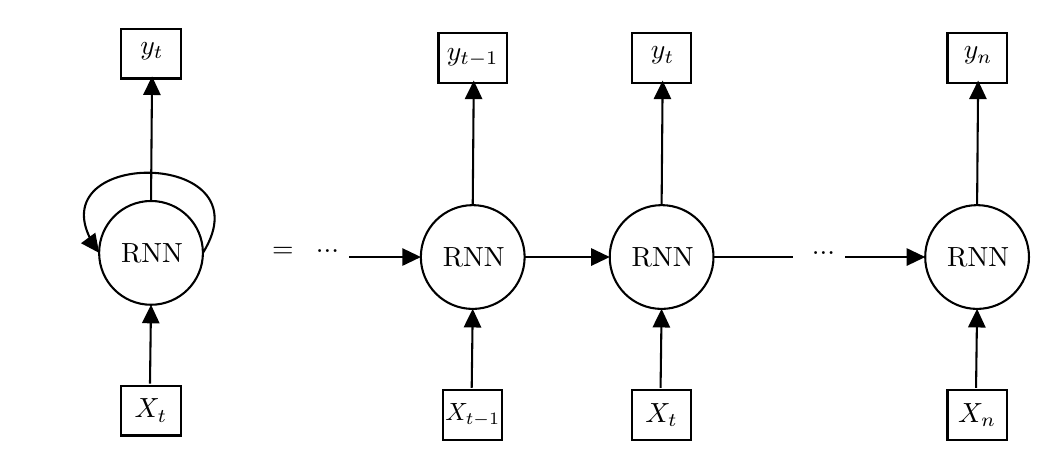
\begin{tikzpicture}[x=0.75pt,y=0.75pt,yscale=-1,xscale=1]
%uncomment if require: \path (0,300); %set diagram left start at 0, and has height of 300

%Shape: Circle [id:dp8533848553232608] 
\draw   (79,153) .. controls (79,139.19) and (90.19,128) .. (104,128) .. controls (117.81,128) and (129,139.19) .. (129,153) .. controls (129,166.81) and (117.81,178) .. (104,178) .. controls (90.19,178) and (79,166.81) .. (79,153) -- cycle ;
%Shape: Rectangle [id:dp3356851682550741] 
\draw   (89.75,217) -- (118.25,217) -- (118.25,241) -- (89.75,241) -- cycle ;
%Shape: Rectangle [id:dp015360643602005286] 
\draw   (89.75,45) -- (118.25,45) -- (118.25,69) -- (89.75,69) -- cycle ;
%Curve Lines [id:da13241738005580928] 
\draw    (77.42,150.74) .. controls (45.07,101.98) and (161.01,101.78) .. (129,153) ;

\draw [shift={(79,153)}, rotate = 233.67] [fill={rgb, 255:red, 0; green, 0; blue, 0 }  ][line width=0.75]  [draw opacity=0] (8.93,-4.29) -- (0,0) -- (8.93,4.29) -- cycle    ;
%Straight Lines [id:da8737873439903896] 
\draw    (103.97,180) -- (103.5,216) ;

\draw [shift={(104,178)}, rotate = 90.75] [fill={rgb, 255:red, 0; green, 0; blue, 0 }  ][line width=0.75]  [draw opacity=0] (8.93,-4.29) -- (0,0) -- (8.93,4.29) -- cycle    ;
%Straight Lines [id:da7493250835057881] 
\draw    (104.48,70) -- (104,128) ;

\draw [shift={(104.5,68)}, rotate = 90.48] [fill={rgb, 255:red, 0; green, 0; blue, 0 }  ][line width=0.75]  [draw opacity=0] (8.93,-4.29) -- (0,0) -- (8.93,4.29) -- cycle    ;
%Shape: Circle [id:dp35751159267212573] 
\draw   (234,155) .. controls (234,141.19) and (245.19,130) .. (259,130) .. controls (272.81,130) and (284,141.19) .. (284,155) .. controls (284,168.81) and (272.81,180) .. (259,180) .. controls (245.19,180) and (234,168.81) .. (234,155) -- cycle ;
%Shape: Rectangle [id:dp2991223335771349] 
\draw   (244.75,219) -- (273.25,219) -- (273.25,243) -- (244.75,243) -- cycle ;
%Shape: Rectangle [id:dp26798597888426934] 
\draw   (242.5,47) -- (275.5,47) -- (275.5,71) -- (242.5,71) -- cycle ;
%Straight Lines [id:da9184227308196455] 
\draw    (258.97,182) -- (258.5,218) ;

\draw [shift={(259,180)}, rotate = 90.75] [fill={rgb, 255:red, 0; green, 0; blue, 0 }  ][line width=0.75]  [draw opacity=0] (8.93,-4.29) -- (0,0) -- (8.93,4.29) -- cycle    ;
%Straight Lines [id:da22975840892719268] 
\draw    (259.48,72) -- (259,130) ;

\draw [shift={(259.5,70)}, rotate = 90.48] [fill={rgb, 255:red, 0; green, 0; blue, 0 }  ][line width=0.75]  [draw opacity=0] (8.93,-4.29) -- (0,0) -- (8.93,4.29) -- cycle    ;
%Shape: Circle [id:dp9315127897645317] 
\draw   (325,155) .. controls (325,141.19) and (336.19,130) .. (350,130) .. controls (363.81,130) and (375,141.19) .. (375,155) .. controls (375,168.81) and (363.81,180) .. (350,180) .. controls (336.19,180) and (325,168.81) .. (325,155) -- cycle ;
%Shape: Rectangle [id:dp6992764849342432] 
\draw   (335.75,219) -- (364.25,219) -- (364.25,243) -- (335.75,243) -- cycle ;
%Shape: Rectangle [id:dp9244658583151169] 
\draw   (335.75,47) -- (364.25,47) -- (364.25,71) -- (335.75,71) -- cycle ;
%Straight Lines [id:da013335644895819732] 
\draw    (349.97,182) -- (349.5,218) ;

\draw [shift={(350,180)}, rotate = 90.75] [fill={rgb, 255:red, 0; green, 0; blue, 0 }  ][line width=0.75]  [draw opacity=0] (8.93,-4.29) -- (0,0) -- (8.93,4.29) -- cycle    ;
%Straight Lines [id:da47760247146100654] 
\draw    (350.48,72) -- (350,130) ;

\draw [shift={(350.5,70)}, rotate = 90.48] [fill={rgb, 255:red, 0; green, 0; blue, 0 }  ][line width=0.75]  [draw opacity=0] (8.93,-4.29) -- (0,0) -- (8.93,4.29) -- cycle    ;
%Straight Lines [id:da7862918954109384] 
\draw    (284,155) -- (323,155) ;
\draw [shift={(325,155)}, rotate = 180] [fill={rgb, 255:red, 0; green, 0; blue, 0 }  ][line width=0.75]  [draw opacity=0] (8.93,-4.29) -- (0,0) -- (8.93,4.29) -- cycle    ;

%Shape: Circle [id:dp5561688511939951] 
\draw   (477,155) .. controls (477,141.19) and (488.19,130) .. (502,130) .. controls (515.81,130) and (527,141.19) .. (527,155) .. controls (527,168.81) and (515.81,180) .. (502,180) .. controls (488.19,180) and (477,168.81) .. (477,155) -- cycle ;
%Shape: Rectangle [id:dp3227398330747131] 
\draw   (487.75,219) -- (516.25,219) -- (516.25,243) -- (487.75,243) -- cycle ;
%Shape: Rectangle [id:dp040272455053374845] 
\draw   (487.75,47) -- (516.25,47) -- (516.25,71) -- (487.75,71) -- cycle ;
%Straight Lines [id:da6201233594039455] 
\draw    (501.97,182) -- (501.5,218) ;

\draw [shift={(502,180)}, rotate = 90.75] [fill={rgb, 255:red, 0; green, 0; blue, 0 }  ][line width=0.75]  [draw opacity=0] (8.93,-4.29) -- (0,0) -- (8.93,4.29) -- cycle    ;
%Straight Lines [id:da35639259950390456] 
\draw    (502.48,72) -- (502,130) ;

\draw [shift={(502.5,70)}, rotate = 90.48] [fill={rgb, 255:red, 0; green, 0; blue, 0 }  ][line width=0.75]  [draw opacity=0] (8.93,-4.29) -- (0,0) -- (8.93,4.29) -- cycle    ;
%Straight Lines [id:da7814656791881325] 
\draw    (375,155) -- (413.5,155) ;


%Straight Lines [id:da5961879457049848] 
\draw    (438.5,155) -- (475,155) ;
\draw [shift={(477,155)}, rotate = 180] [fill={rgb, 255:red, 0; green, 0; blue, 0 }  ][line width=0.75]  [draw opacity=0] (8.93,-4.29) -- (0,0) -- (8.93,4.29) -- cycle    ;

%Straight Lines [id:da20737537017177732] 
\draw    (199.5,155) -- (232,155) ;
\draw [shift={(234,155)}, rotate = 180] [fill={rgb, 255:red, 0; green, 0; blue, 0 }  ][line width=0.75]  [draw opacity=0] (8.93,-4.29) -- (0,0) -- (8.93,4.29) -- cycle    ;


% Text Node
\draw (104,229) node   {$X_{t}$};
% Text Node
\draw (104.5,56) node   {$y_{t}$};
% Text Node
\draw (104.5,153) node  [align=left] {RNN};
% Text Node
\draw (167.5,153) node   {$=$};
% Text Node
\draw (259,231) node [scale=0.9]  {$X_{t-1}$};
% Text Node
\draw (259,59) node   {$y_{t-1}$};
% Text Node
\draw (259.5,155) node  [align=left] {RNN};
% Text Node
\draw (350,231) node   {$X_{t}$};
% Text Node
\draw (350.5,58) node   {$y_{t}$};
% Text Node
\draw (350.5,155) node  [align=left] {RNN};
% Text Node
\draw (502,231) node   {$X_{n}$};
% Text Node
\draw (502.5,58) node   {$y_{n}$};
% Text Node
\draw (502.5,155) node  [align=left] {RNN};
% Text Node
\draw (428,153) node   {$...$};
% Text Node
\draw (189,152) node   {$...$};


\end{tikzpicture}

\caption{A graphical illustration of the RNN cell. The self-connected edge in the left hand side denotes the temporal nature we unroll on the right side. The cell takes as input a state vector and an input vector at time t, and outputs a prediction and the new state vector used for the next prediction. Internally the simplest form this operation takes is to concatenate the state vector with the input and use an ordinary dense network as described in section \ref{sec:ANN} trained with back-propagation.}\label{fig:rnn}
\end{figure}